\section{Building Block View}

In this section we will describe the \gls{app} using some elements of the 4+1 Architectural View Model. With this model we
aim to target an understanding of all our main stakeholders.

We will use 4 different views, which should focus on specific elements of the project. Each view provides a different
purpose \cite{refart:KR41}. For this project we will provide the 3 following views of the 4+1 Architectural View 
Model:

\begin{itemize}
    \item \textbf{Scenario view}: simple description for the end user 
    \item \textbf{Structural view}: object-oriented decomposition
    \item \textbf{Behavior view}: description of the existing processes
\end{itemize}

\subsection{Scenario view}

Our first picture \ref{fig:preliminary_use_case} provided our stakeholders a brief presentation of the basic functionalities of our app. Other elements addressed in this view were presented in the chapter where we discussed the business context, \ref{business_context}. 

An example on how each feature of the app should work can be found in our use case in section \ref{table_use_case}.
More elements of this view will be presented while discussing the internal decisions in chapter \ref{Patterns_Tacticts}. 

\subsection{Structural view}

For the following graphic we choose a \gls{class diagram} to provide our development team a further view of the
structural elements of the project. This first class diagram gives a simple description of the classes that can
exist in the app.

\begin{figure}[H]
    \centering
    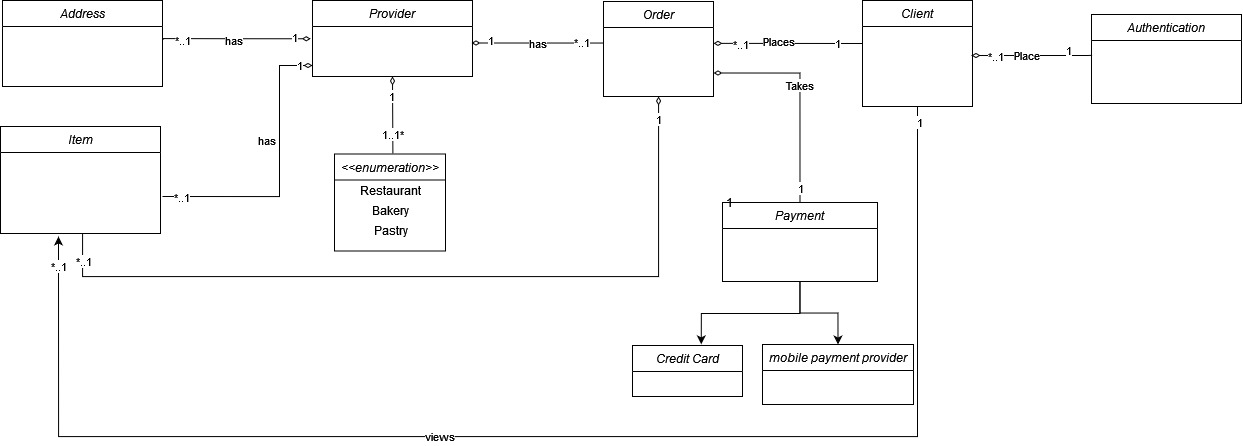
\includegraphics[width=0.6\textwidth]{assets/simple_classes_CD.jpg}
    \caption{Level 1 - Class Diagramm}
    \label{fig:simple_class_diagram}
\end{figure}

\newpage
\thispagestyle{lscape}
\begin{landscape}

Zooming down the classes we presented before, we can see how they are build with its attributes, methods and
interaction with other elements.

\begin{figure}[H]
    \centering
    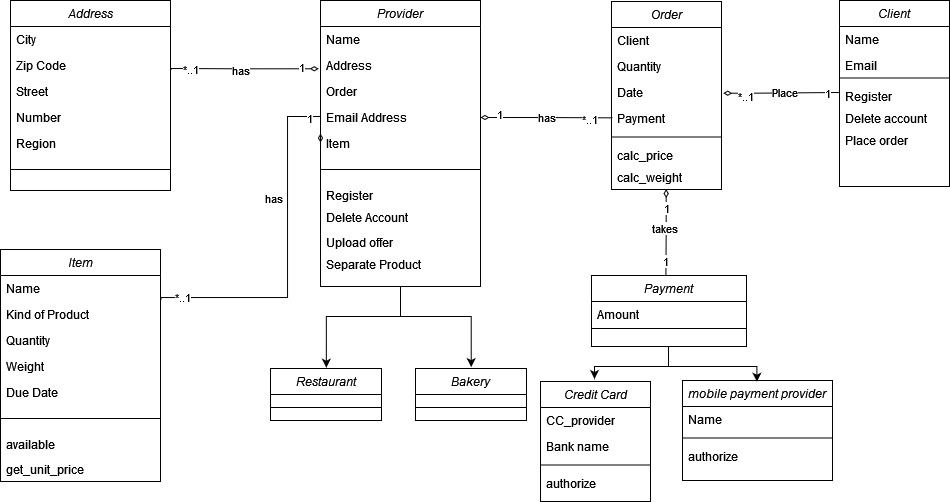
\includegraphics[width=1.5\textwidth]{assets/classes_CD.jpg}
    \caption{Classes Overview}
    \label{fig:class_CD}
\end{figure}

\end{landscape}

\subsection{Behavior view}

The following \gls{activity diagram} depicts the register and login procedure within the app. It should explain our
main stakeholders, \glsplural{provider} and \glsplural{client}, the starting process of the app.

\begin{figure}[H]
    \centering
    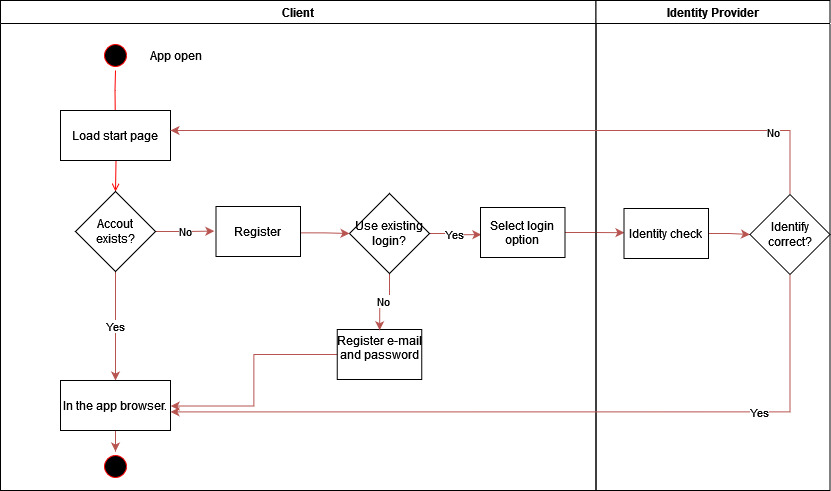
\includegraphics[width=1\textwidth]{assets/login_AC.jpg}
    \caption{Login procedures}
    \label{fig:login_register}
\end{figure}

To help understanding the above process we created the following \gls{sequence diagram} that depict the communication flow 
with the third party providers. 

\begin{figure}[H]
    \centering
    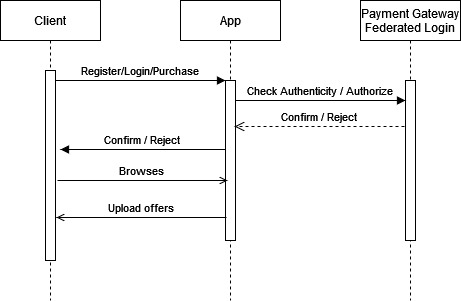
\includegraphics[width=0.7\textwidth]{assets/sequence_login_payment.jpg}
    \caption{Sequence of actions with third party applications}
    \label{fig:sequence_login_payment}
\end{figure}



